\clearpage
\begin{flushright}
	\textit{Лекция №6}
	\textit{2016.03.28}
\end{flushright}

\lstinputlisting[language=c, label=code_read_proc, caption=Пример процедуры чтения]{listing/1.c} 

В \ref{code_read_proc} создаем 1 функцию \verb|copy_to_user| (эта функция на первом этапе выполняет вызов ф-и \verb|access_ok()| )

Функция \verb|access_ok(type, addr, size)|   проверяет, действительно ли существует указатель на пространство пользователя, к которому необходимо получить доступ. Вызывается в тексте функции. Имеет 3 параметра: указатель на начала блока памяти, размер блока и права доступа. type: \verb|VERIFY_READ|  или \verb|VERIFY_WRITE| (предполагает  \verb|VERIFY_READ|). Адресное пространство процессов защищены и виртуальны. ФС proc позволяет взаимодействовать с адресным пространством ядра и делается это через буфера. Буфера могут быть объявлены как указатель на buf или на page. 

Загружаемые модули ядра пишутся по определенным правилам: в текст модуля обязательно должны быть включены два макроса (\verb|module_init| \verb|module_exit|: они регистрируют нашу функцию). Макросы вставляются в текст. В отличии от функций, которые имеют собственное адреcное пространство, макросы являются вставками в текст какой то программы, мы не перекомпилируем ядро, но тем не менее это вставка. В разных примерах по разному регистрируются call-back функции. Тут, функция read (наша, чтения виртуального файла) регистрируется через ???
Необязательно использовать \verb|copy_to_user| (пример - когда используется \verb|mem_copy()|).  Существуют разные способы взаимодействия с виртуальными файлами: есть ФС proc, есть ФС procfs.
Кроме \verb|copy_to_user()| \verb|copy_from_user()| упоминаются еще \verb|get_user()| \verb|put_user()|.

\lstinputlisting[language=c, label=code_mem_copy, caption={Пример, когда используется mem\_copy()}]{listing/2.c} 

В \ref{code_mem_copy} - пример создания файла в proc. Для функции write должны обеспечить импортирование данных, так как они приходят из пространства пользователя. Для функции read , т.к. данные уже находятся в пространстве ядра. 

\lstinputlisting[language=c, label=code_define_proc_dir_entry, caption={Еще пример}]{listing/3.c}

В \ref{code_define_proc_dir_entry} видим определение полей структуры \verb|proc_dir_entry|.

В самом тексте фортунок используется \verb|sprintf()| (по тем же соображениям что и \verb|mem_copy|). Сами фортунки служат вспомогательным примером.

\chapter{Взаимоисключения ядра}

(после этого будем рассматривать прерывания и пример драйвера. Драйвер реализуется в виде загружаемого модуля ядра и самым распространенным примером является пример USB hid driver)

Примером, на сколько важен монопольный доступ к разделяемым данным, является взаимодейсвтие паралельных процессов (безразлично квази или реально параллельные).

\paragraph{Пример, когда два параллельных  процесса пытаются добавить в очередь новый элемент}

Каждый из процессов пытаются записать в очередь (связный список) свою структуру
\begin{lstlisting}[language=c, caption=Структура queue]
struct queue {
	int data;
	struct queue *next;
}
\end{lstlisting}


\begin{table}[H]
\begin{tabular}{|l|l|}
\hline
p1: & p2: \\
\hline
new(a); & \\
a->next = q->next;  & \\
\hline
\multicolumn{2}{|c|}{прервали p1} \\
\hline
 & new(b); \\
 & b->next = q->next; \\
 & q->next = b; \\
\hline
\multicolumn{2}{|c|}{возобновили p1} \\
\hline
q->next = a; & \\
\hline
\end{tabular}
\end{table}

\begin{figure}[H]
  \centering
  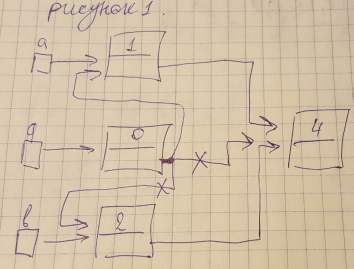
\includegraphics[width=\textwidth]{pic/1.png}
  \caption{pic}
\end{figure}

Необходимо предоставлять монопольный доступ.

Спин блокировки – строятся на основе команды \verb|test_and_set| или \verb|test_and_set_lock|. Lock – слово в памяти.




